\documentclass{article} 
\usepackage[left=0.75in,top=0.6in,right=0.75in,bottom=0.6in]{geometry} % Document margins
\usepackage{tabularx}
\usepackage{fancyvrb}
%\usepackage[hidelinks]{hyperref}
\usepackage{graphicx}
\usepackage{float}
\usepackage{fancyhdr}
\usepackage{geometry}
\usepackage{lastpage}
\usepackage{tabu}
\usepackage{hyperref}

\geometry{
  top=1in,            % <-- you want to adjust this
  inner=0.5in,
  outer=0.5in,
  bottom=1in,
  headheight=5ex,       % <-- and this
  headsep=4ex,          % <-- and this
}

\pagestyle{fancy}
\fancyhf{}
\rhead{\Large\textit{Old Dominion University}}
\lhead{\Large\textit{ECE 432: Assignment 8}}
\cfoot{Page \thepage \hspace{1pt} of \pageref{LastPage}}
\renewcommand{\footrulewidth}{1pt}

\begin{document}

%----------------------------------------------------------------------------------------
%		 TITLE PAGE
%----------------------------------------------------------------------------------------

\begin{titlepage}

\vspace*{45 pt}
\begin{center}
\Huge{\bf CS 432/532:  Web Science}\\
\huge{Spring 2017\\}

\vspace{60 pt}
\Huge\underline {Assignment 8}\\

\vspace{10 pt}
\Huge{Michael Micros}\\\

{\Large \bf {Instructor: Michael L. Nelson}}\\

\vspace{230 pt}
{\huge \bf {Old Dominon University}}\\
{\huge \bf {Norfolk, Virginia}}\\

\vspace{10 pt}
\today

\end{center}
\end{titlepage}




%----------------------------------------------------------------------------------------
%		PROBLEM 1
%----------------------------------------------------------------------------------------

\section*{{\underline{\huge {Problem 1:}} Generating blog-term matrix  }}
In order to generate the blog term matrix that is used throughout this assignment, it was first necessary to get 100 unique blogs. The ``part1.py'' script accomplishes this by making use of ``urllib2'' and ``BeautifulSoup''. The way it works is we make a request for the ``next blog" and once we get a ``200 OK'', we iterate through all of the blog's pages and add them to the ``feedlist.txt" which will later be given to the feedparser script. A summary of the blog title and number of pages is saved in ``blogstats.txt".

\begin{figure}[H]
 \centering
 	\includegraphics[height=8cm]{P1.png}
  \caption{Section of ``part1.py"}
\end{figure}


\begin{figure}[H]
 \centering
 	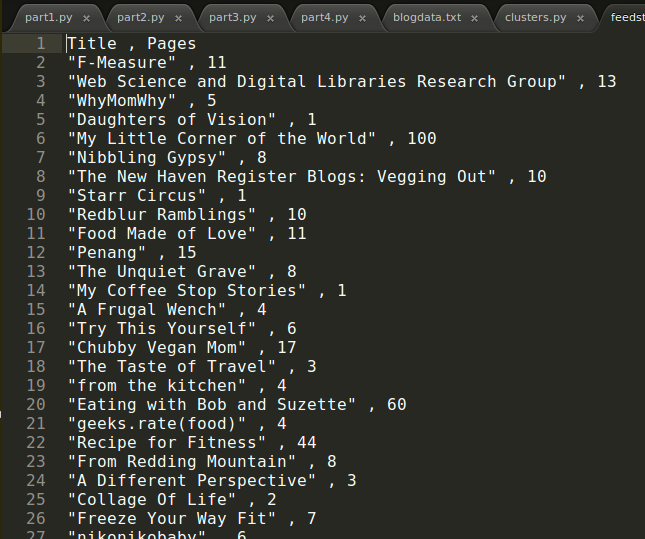
\includegraphics[height=9cm]{feddstats.png}
  \caption{Part of the blog data collected}
\end{figure}

Once all the blog data is collected, it is fed to the feedparser introduced in Chapter 3 of the ``Collective Intelligence Programming", which created the blog-term matrix where every row represents a blog and every column represents 1 of the 1000 most common words across all blogs.



%----------------------------------------------------------------------------------------
%		PROBLEM 2
%----------------------------------------------------------------------------------------

\section*{{\underline{\huge {Problem 2:}} Creating a dendrogram  }}
The rest of this assignments makes heavy  use of the ``clusters.py" script and its functions provided in the ``Collective Intelligence Programming" textbook.

\begin{figure}[H]
 \centering
 	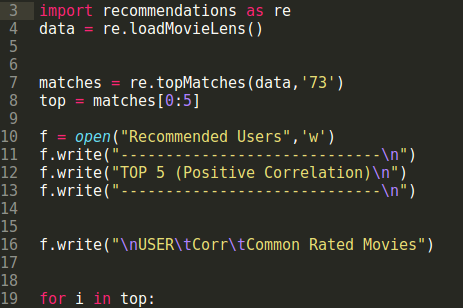
\includegraphics[height=4cm]{p2.png}
  \caption{``part2.py""}
\end{figure}

The dendrogram of the collected blogs is displayed on the next page. Obviously it is not easily readable, but the top half of the dendrogram represents two big glusters for lifestyle and food , which are all pretty similar to each other which explains the layout. Additionally, there are smaller clusters toward the bottom having to do with coffee, art, travel, education/programming, etc.

\begin{figure}[H]
 \centering
 	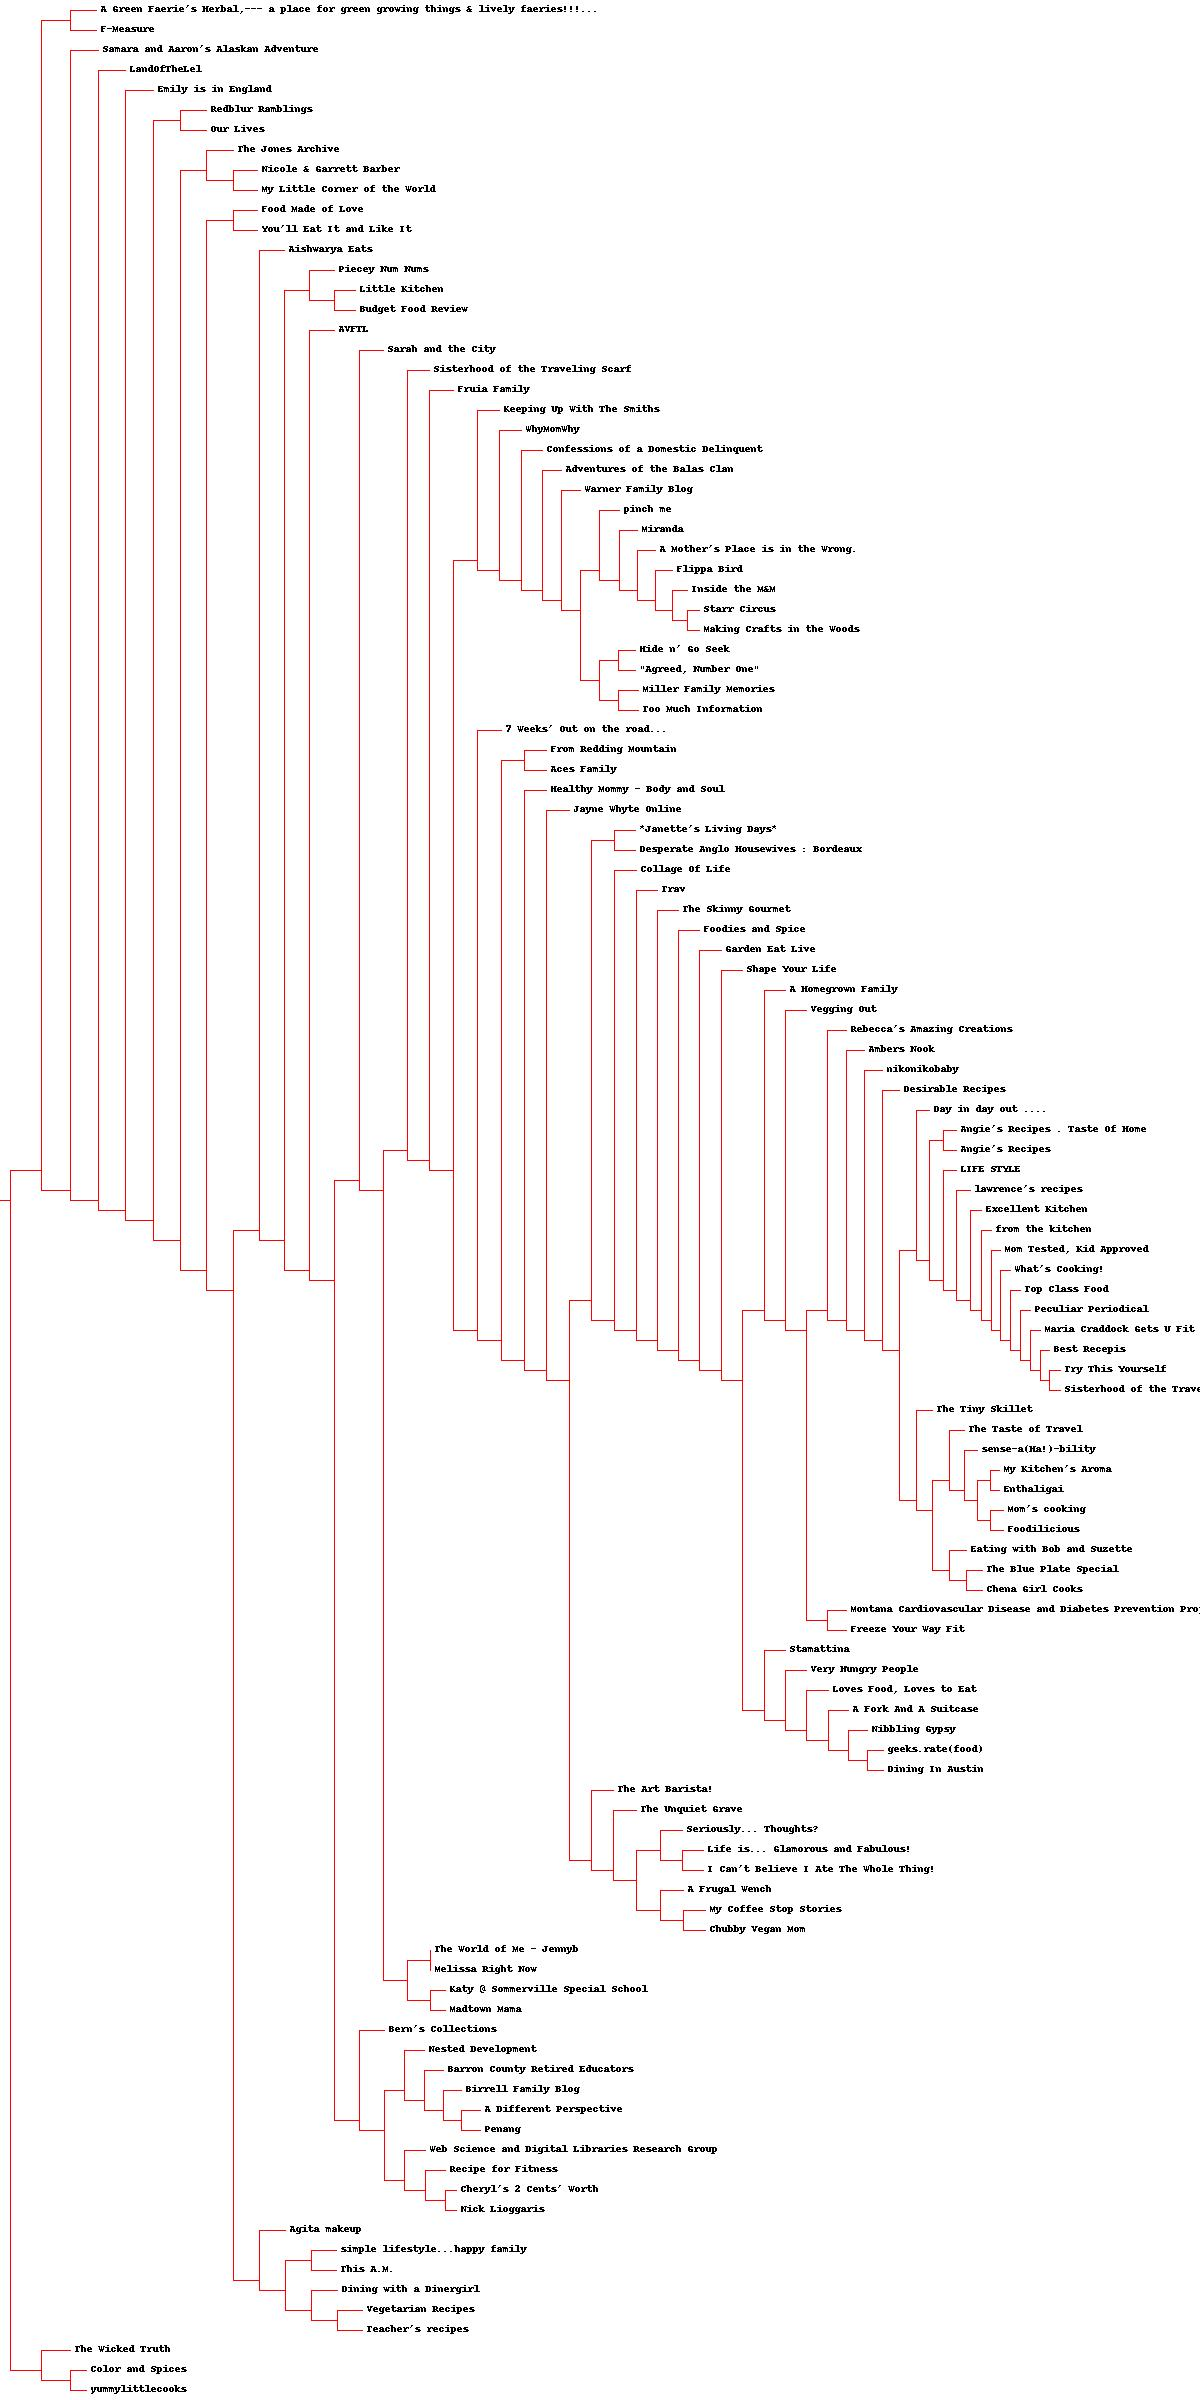
\includegraphics[height=22cm]{clusters.jpg}
  \caption{Dendrogram of collected blogs}
\end{figure}

%----------------------------------------------------------------------------------------
%		PROBLEM 3
%----------------------------------------------------------------------------------------

\section*{{\underline{\huge {Problem 3:}} Clustering using K-Means }}

In order to get the desired results the ``kclusters'' function in the ``clusters.py script" was used 3 times for k=5,10 and 20.
The number of iterations needed for 5 clusters was 8. 6 iterations were needed to generate 10 clusters, and 4 iterations to get 20 clusters. 


\begin{figure}[H]
 \centering
 	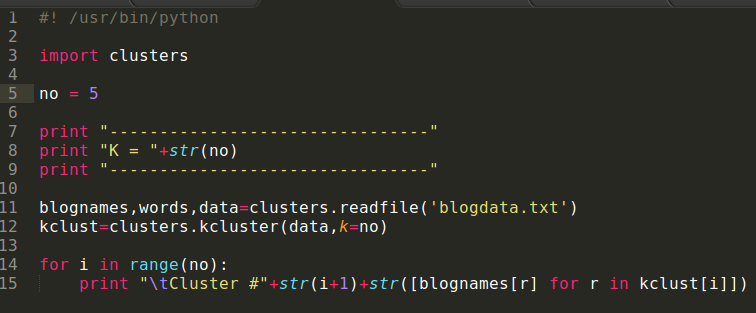
\includegraphics[height=7cm]{p3.png}
  \caption{``part3.py""}
\end{figure}

\begin{figure}[H]
 \centering
 	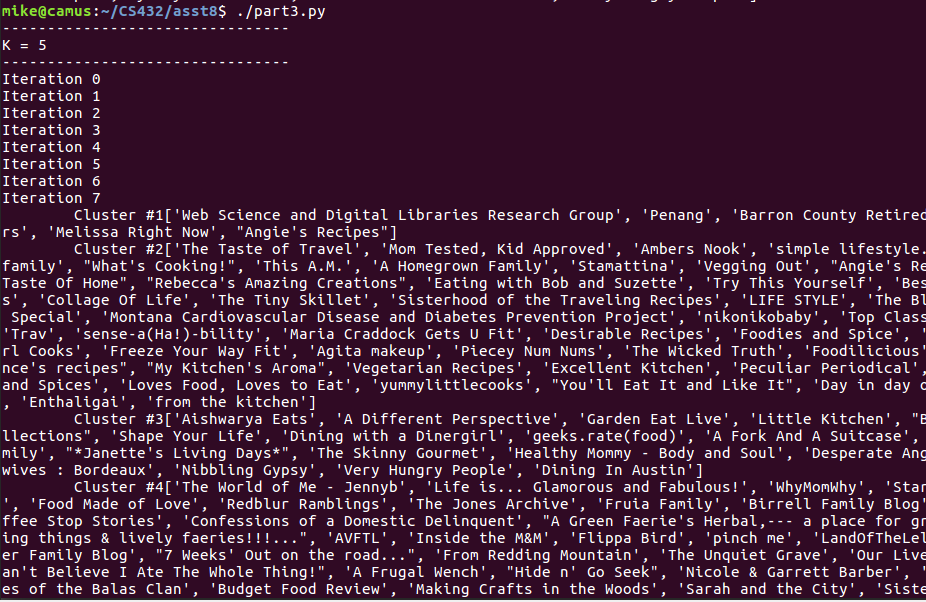
\includegraphics[height=10cm]{q3k5.png}
  \caption{Results for K-Means with k=5}
\end{figure}

\begin{figure}[H]
 \centering
 	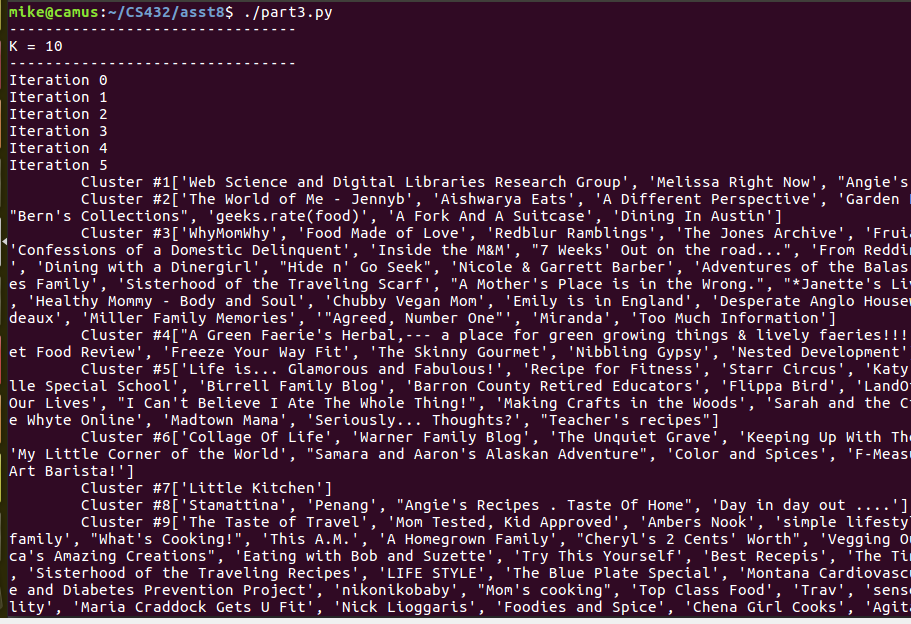
\includegraphics[height=10cm]{q3k10.png}
  \caption{Results for K-Means with k=10}
\end{figure}

\begin{figure}[H]
 \centering
 	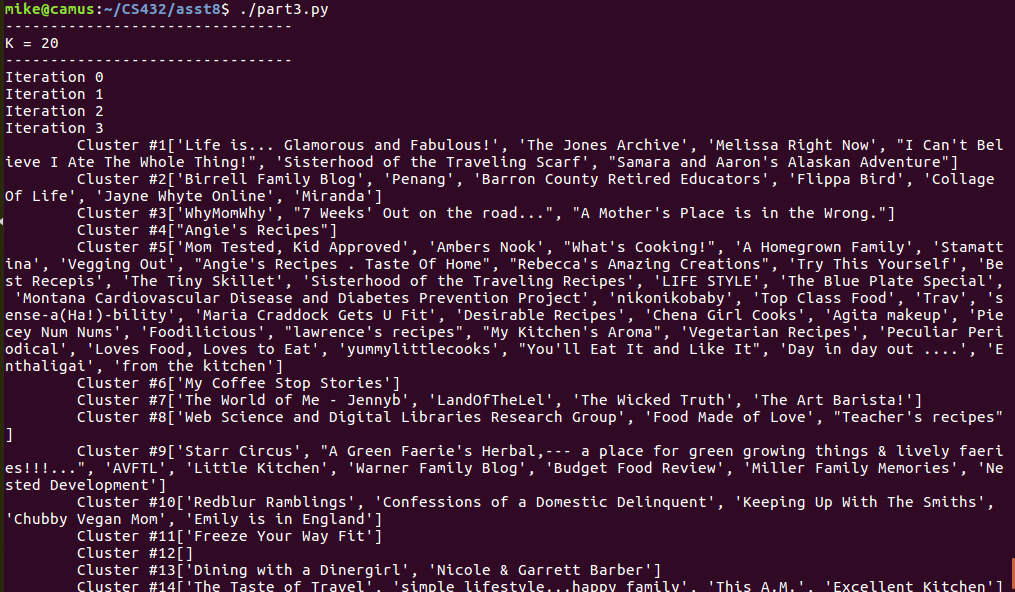
\includegraphics[height=10cm]{q3k20.png}
  \caption{Results for K-Means with k=20}
\end{figure}



%----------------------------------------------------------------------------------------
%		PROBLEM 4
%----------------------------------------------------------------------------------------

\section*{{\underline{\huge {Problem 4:}}}  2D display using Multidimentional Scaling}
In order to perform multidimensional scaling the ``scaledown'' and  ``draw2d'' functions were used from the ``clusters.py script'', as is seen below.

\begin{figure}[H]
 \centering
 	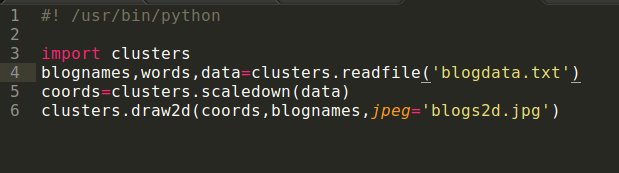
\includegraphics[height=4cm]{p4.png}
  \caption{``part4.py""}
\end{figure}

Again the results are not easily visible but the graph upon analysis has 2 easily distinguishable groups. The  blogs in the bottom left correspond to the ``lifestyle'' blogs whereas the blogs on the top half and also the right mainly are ``food"  blogs. In total, 136 iterations were required going from an average total difference of 6733.3 (potatos?) to 4257.7.

\begin{figure}[H]
 \centering
 	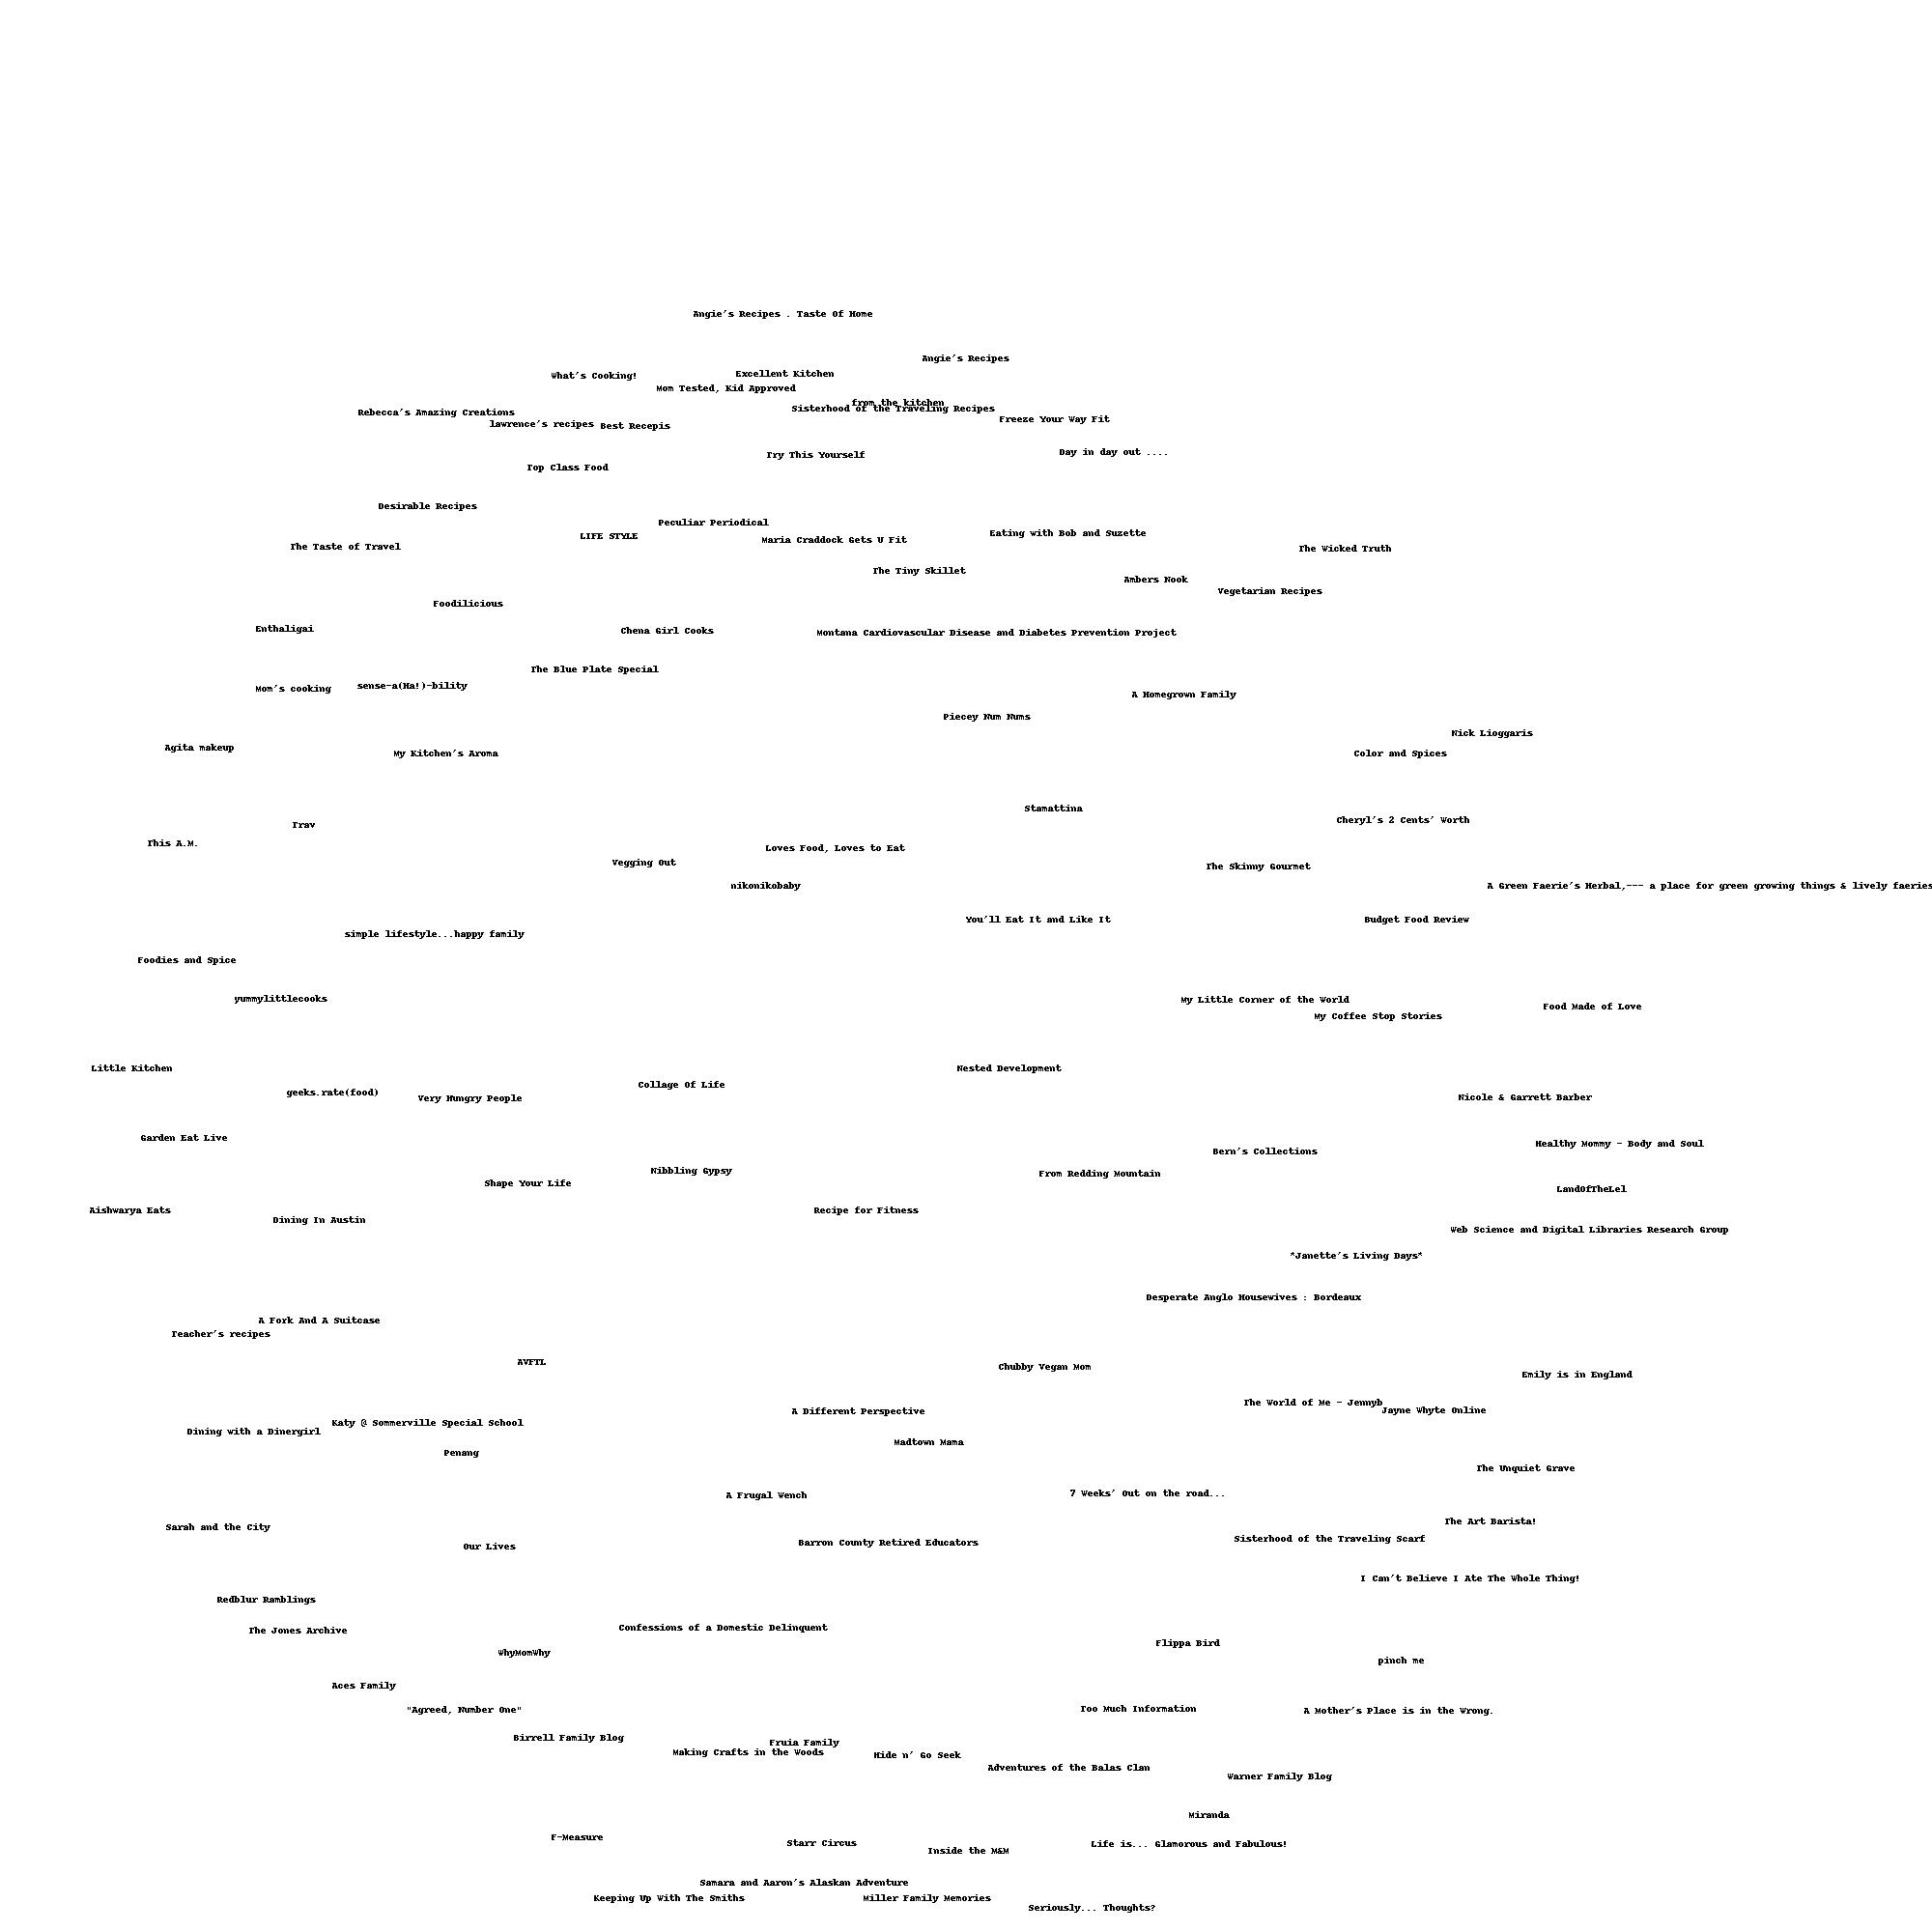
\includegraphics[height=16cm]{MDS.jpg}
  \caption{2D display of our blog data}
\end{figure}


%----------------------------------------------------------------------------------------
\end{document}
